\documentclass[12pt,a4paper]{amsart}
\usepackage{amsfonts}
\usepackage{amsthm}
\usepackage{amsmath}
\usepackage{amscd}
\usepackage[latin2]{inputenc}
\usepackage{t1enc}
\usepackage{xcolor}
\usepackage{listings}
\usepackage{tikz}
\usepackage[mathscr]{eucal}
\usepackage{indentfirst}
\usepackage{graphicx}
\usepackage{graphics}
\usepackage{pict2e}
\usepackage{epic}
\numberwithin{equation}{section}
\usepackage[margin=2.9cm]{geometry}
\usepackage{epstopdf} 

 \def\numset#1{{\\mathbb #1}}

 
\renewcommand{\familydefault}{\sfdefault}

\theoremstyle{plain}
\newtheorem{Th}{Theorem}[section]
\newtheorem{Lemma}[Th]{Lemma}
\newtheorem{Cor}[Th]{Corollary}
\newtheorem{Prop}[Th]{Proposition}

 \theoremstyle{definition}
\newtheorem{Def}[Th]{Definition}
\newtheorem{Conj}[Th]{Conjecture}
\newtheorem{Rem}[Th]{Remark}
\newtheorem{?}[Th]{Problem}
\newtheorem{Ex}[Th]{Example}

\newcommand{\im}{\operatorname{im}}
\newcommand{\Hom}{{\rm{Hom}}}
\newcommand{\diam}{{\rm{diam}}}
\newcommand{\ovl}{\overline}
%\newcommand{\M}{\mathbb{M}}


\tikzset{every picture/.style={line width=0.75pt}} %set default line width to 0.75pt        

\definecolor{mGreen}{rgb}{0,0.6,0}
\definecolor{mGray}{rgb}{0.5,0.5,0.5}
\definecolor{mPurple}{rgb}{0.58,0,0.82}
\definecolor{backgroundColour}{rgb}{0.95,0.95,0.92}

\lstdefinestyle{CStyle}{
    backgroundcolor=\color{backgroundColour},   
    commentstyle=\color{mGreen},
    keywordstyle=\color{magenta},
    numberstyle=\tiny\color{mGray},
    stringstyle=\color{mPurple},
    basicstyle=\footnotesize,
    breakatwhitespace=false,         
    breaklines=true,                 
    captionpos=b,                    
    keepspaces=true,                 
    numbers=left,                    
    numbersep=5pt,                  
    showspaces=false,                
    showstringspaces=false,
    showtabs=false,                  
    tabsize=2,
    language=C
}

\begin{document}

\title{HDF5 vary number of processes on restart}

\maketitle

\section{The topology of datasets}

\begin{figure}[ht]


\tikzset{every picture/.style={line width=0.75pt}} %set default line width to 0.75pt        

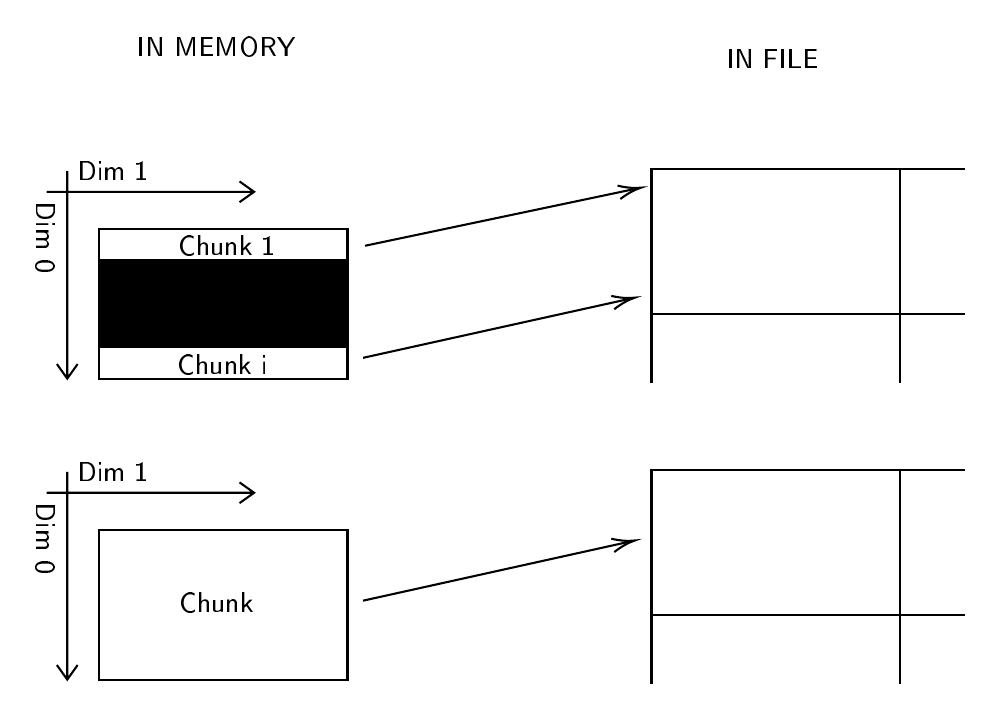
\begin{tikzpicture}[x=0.75pt,y=0.75pt,yscale=-1,xscale=1]
%uncomment if require: \path (0,374); %set diagram left start at 0, and has height of 374

%Shape: Axis 2D [id:dp09251878516164269] 
\draw  (51,95) -- (51,195)(141,105) -- (41,105) (56,188) -- (51,195) -- (46,188) (134,100) -- (141,105) -- (134,110)  ;
%Shape: Rectangle [id:dp2426843170893367] 
\draw   (66.5,123) -- (186,123) -- (186,138) -- (66.5,138) -- cycle ;
%Shape: Rectangle [id:dp8338475867508441] 
\draw   (66.5,180) -- (186,180) -- (186,195) -- (66.5,195) -- cycle ;
%Shape: Rectangle [id:dp7145458164212026] 
\draw  [fill={rgb, 255:red, 0; green, 0; blue, 0 }  ,fill opacity=1 ] (66.5,138) -- (186,138) -- (186,180) -- (66.5,180) -- cycle ;
%Straight Lines [id:da4034657837382658] 
\draw    (194.5,131) -- (325.54,103.41) ;
\draw [shift={(327.5,103)}, rotate = 528.11] [color={rgb, 255:red, 0; green, 0; blue, 0 }  ][line width=0.75]    (10.93,-3.29) .. controls (6.95,-1.4) and (3.31,-0.3) .. (0,0) .. controls (3.31,0.3) and (6.95,1.4) .. (10.93,3.29)   ;

%Shape: Rectangle [id:dp6686060061970889] 
\draw   (332.5,94) -- (452,94) -- (452,164) -- (332.5,164) -- cycle ;
%Straight Lines [id:da5420092360319286] 
\draw    (332.5,164) -- (332.5,197) ;


%Straight Lines [id:da7588623066244546] 
\draw    (452,164) -- (452,197) ;


%Straight Lines [id:da1810735040320477] 
\draw    (452,164) -- (483.5,164) ;


%Straight Lines [id:da1362684037747448] 
\draw    (452,94) -- (483.5,94) ;


%Straight Lines [id:da2013361520865684] 
\draw    (193.5,185) -- (322.55,156.43) ;
\draw [shift={(324.5,156)}, rotate = 527.52] [color={rgb, 255:red, 0; green, 0; blue, 0 }  ][line width=0.75]    (10.93,-3.29) .. controls (6.95,-1.4) and (3.31,-0.3) .. (0,0) .. controls (3.31,0.3) and (6.95,1.4) .. (10.93,3.29)   ;

%Shape: Axis 2D [id:dp8479181396324231] 
\draw  (51,240) -- (51,340)(141,250) -- (41,250) (56,333) -- (51,340) -- (46,333) (134,245) -- (141,250) -- (134,255)  ;
%Shape: Rectangle [id:dp08827249058943654] 
\draw   (66.5,268) -- (186,268) -- (186,340) -- (66.5,340) -- cycle ;
%Shape: Rectangle [id:dp38563479487780983] 
\draw   (332.5,239) -- (452,239) -- (452,309) -- (332.5,309) -- cycle ;
%Straight Lines [id:da7536094957580308] 
\draw    (332.5,309) -- (332.5,342) ;


%Straight Lines [id:da3286778972193569] 
\draw    (452,309) -- (452,342) ;


%Straight Lines [id:da5464056706763105] 
\draw    (452,309) -- (483.5,309) ;


%Straight Lines [id:da5453076101928134] 
\draw    (452,239) -- (483.5,239) ;


%Straight Lines [id:da1890183290117633] 
\draw    (193.5,302) -- (322.55,273.43) ;
\draw [shift={(324.5,273)}, rotate = 527.52] [color={rgb, 255:red, 0; green, 0; blue, 0 }  ][line width=0.75]    (10.93,-3.29) .. controls (6.95,-1.4) and (3.31,-0.3) .. (0,0) .. controls (3.31,0.3) and (6.95,1.4) .. (10.93,3.29)   ;


% Text Node
\draw (73,95) node  [align=left] {Dim 1};
% Text Node
\draw (41,127) node [rotate=-90] [align=left] {Dim 0};
% Text Node
\draw (126,188) node  [align=left] {Chunk i};
% Text Node
\draw (128,131) node  [align=left] {Chunk 1};
% Text Node
\draw (73,240) node  [align=left] {Dim 1};
% Text Node
\draw (41,272) node [rotate=-90] [align=left] {Dim 0};
% Text Node
\draw (123,303) node  [align=left] {Chunk};
% Text Node
\draw (123,35) node  [align=left] {IN MEMORY};
% Text Node
\draw (391,41) node  [align=left] {IN FILE};


\end{tikzpicture}

\caption{2-Dim grid example}
\label{fig:2dgrid}
\end{figure}

The datasets may be allocated completely contiguous or partly
contiguous. For the first case, we can write the whole region at once to
the file. For this, we have to create a memoryspace and a filespace:
\begin{lstlisting}[style=CStyle]
memory_space = H5Screate_simple(rank_m, dims_memory, NULL);
file_space = H5Screate_simple(rank_f, dims_file, NULL);
\end{lstlisting}
where {\tt rank\_m}, or {\tt rank\_f},  is the dimensionality of the selected region and
{\tt dims\_memory} and {\tt dims\_file} an array that keeps the number of
elements for each dimension.

If we have a completely contiguous region, {\tt rank\_m} and 
{\tt rank\_f}, are identical. If we have partly contiguous regions, 
the ranks may differ. Most likely for partly contiguous regions
is the case, that we have only one dimension of a multi dimensional
array contiguous (for instance the rows in a 2-dim array in C, compare
fig. \ref{fig:rowmajor}, or contiguous columns in Fortran). 

In order to avoid too much complexity, we will support only datasets,
that are not fragmented in the dimensions. That means, we will support
only either completely contiguous regions or partly contiguous regions
which are fully contiguous inside the sub dimensions. Thus, it is
sufficient to define an {\tt~offset} and a {\tt~count} property.

The offset and count properties always have the dimensionality of the
shared dataset. For instance, considering a rank local and partly
contiguous 2-dim dataset which is stored in an array where 
only the rows are contiguous in memory. We can define:
\begin{lstlisting}[style=CStyle]
offset = { off_row, off_col }
count  = { 0, cnt_col } // row contiguous -> cnt_row = 0
\end{lstlisting}

Having the file- and memoryspace set and also the count and offset
property, we can create the dataset inside the file and select the 
dataset corresponding file region with:
\begin{lstlisting}[style=CStyle]
dset_id = H5Dcreate(file_id, dataset_name, hdf5_datatype, 
            file_space, H5P_DEFAULT, H5P_DEFAULT, H5P_DEFAULT);
H5Sselect_hyperslab(file_space, H5S_SELECT_SET, offset, NULL, 
            count, NULL);
\end{lstlisting}
And finally write the dataset with:
\begin{lstlisting}[style=CStyle]
H5Dwrite(dset_id, hdf5_datatype, memory_space, file_space, 
            plist_id, data);
\end{lstlisting}


\section{Taking care of ghost cells}
\begin{figure}[ht]
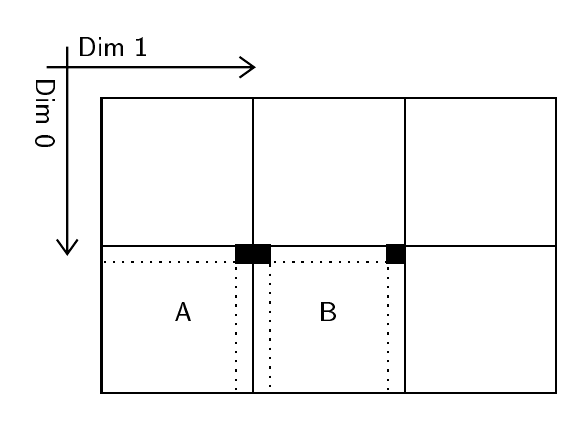
\begin{tikzpicture}[x=0.75pt,y=0.75pt,yscale=-1,xscale=1]
%uncomment if require: \path (0,300); %set diagram left start at 0, and has height of 300

%Shape: Rectangle [id:dp7623273016364707] 
\draw   (51.5,151) -- (124.5,151) -- (124.5,222) -- (51.5,222) -- cycle ;
%Shape: Rectangle [id:dp4868977393130458] 
\draw   (51.5,80) -- (124.5,80) -- (124.5,151) -- (51.5,151) -- cycle ;
%Shape: Rectangle [id:dp7992870896708093] 
\draw   (124.5,80) -- (197.5,80) -- (197.5,151) -- (124.5,151) -- cycle ;
%Shape: Rectangle [id:dp4346528285505409] 
\draw   (124.5,151) -- (197.5,151) -- (197.5,222) -- (124.5,222) -- cycle ;
%Shape: Rectangle [id:dp7385891406488625] 
\draw   (197.5,80) -- (270.5,80) -- (270.5,151) -- (197.5,151) -- cycle ;
%Shape: Rectangle [id:dp6337817779956811] 
\draw   (197.5,151) -- (270.5,151) -- (270.5,222) -- (197.5,222) -- cycle ;
%Shape: Axis 2D [id:dp07711264299760034] 
\draw  (35,55) -- (35,155)(125,65) -- (25,65) (40,148) -- (35,155) -- (30,148) (118,60) -- (125,65) -- (118,70)  ;
%Shape: Rectangle [id:dp7057870116196296] 
\draw  [dash pattern={on 0.84pt off 2.51pt}] (51.5,151) -- (124.5,151) -- (124.5,159) -- (51.5,159) -- cycle ;
%Shape: Rectangle [id:dp14503576341423963] 
\draw  [dash pattern={on 0.84pt off 2.51pt}] (124.5,151) -- (197.5,151) -- (197.5,159) -- (124.5,159) -- cycle ;
%Shape: Rectangle [id:dp8866120660824588] 
\draw  [dash pattern={on 0.84pt off 2.51pt}] (132.5,151) -- (132.5,222) -- (124.5,222) -- (124.5,151) -- cycle ;
%Shape: Rectangle [id:dp9099321872455894] 
\draw  [dash pattern={on 0.84pt off 2.51pt}] (124.5,151) -- (124.5,222) -- (116.5,222) -- (116.5,151) -- cycle ;
%Shape: Rectangle [id:dp11377940801055231] 
\draw  [dash pattern={on 0.84pt off 2.51pt}] (197.5,151) -- (197.5,222) -- (189.5,222) -- (189.5,151) -- cycle ;
%Shape: Square [id:dp4016938424905261] 
\draw  [fill={rgb, 255:red, 0; green, 0; blue, 0 }  ,fill opacity=1 ] (116.25,150.75) -- (124.75,150.75) -- (124.75,159.25) -- (116.25,159.25) -- cycle ;
%Shape: Square [id:dp7458528516768157] 
\draw  [fill={rgb, 255:red, 0; green, 0; blue, 0 }  ,fill opacity=1 ] (124.25,150.75) -- (132.75,150.75) -- (132.75,159.25) -- (124.25,159.25) -- cycle ;
%Shape: Square [id:dp46350377922873665] 
\draw  [fill={rgb, 255:red, 0; green, 0; blue, 0 }  ,fill opacity=1 ] (189.25,150.75) -- (197.75,150.75) -- (197.75,159.25) -- (189.25,159.25) -- cycle ;

% Text Node
\draw (91,183) node  [align=left] {A};
% Text Node
\draw (161,183) node  [align=left] {B};
% Text Node
\draw (57,55) node  [align=left] {Dim 1};
% Text Node
\draw (25,87) node [rotate=-90] [align=left] {Dim 0};


\end{tikzpicture}

\caption{2-Dim grid example}
\label{fig:rowmajor}
\end{figure}

I order to restart with a different amount of processes, we need to have
the pure data inside the cp file. That is, data, excluding the ghost
cells.

The user may specify the ghost cells by the matrix $g$. For every
dimension $d$ of an $m$ dimensional dataset, $g$ keeps two integer
scalars, $I$ and $F$:
\begin{equation}
g_{d} = (I, F)
\end{equation}
With this, $g_{d0}$ spezifies if the dimension $d$ has a neighboring
domain in
index decreasing direction, plus, the protected
dataset has $I$ ghostcells included in the allocation ($g_{d1}$ analog).

\ref{fig:2dgrid} shows an example of a 2 dimansional grid. In that case
we have for g:
\begin{eqnarray*}
g^{(A)}_0 = (0,1) \quad , \quad g^{(A)}_1 = (0,1) \\
g^{(B)}_0 = (1,1) \quad , \quad g^{(B)}_1 = (0,1)
\end{eqnarray*}

Inside the implementation, this gives us the posibility to write the
data and excluding the ghost cells:

\begin{lstlisting}[style=CStyle]
/**
 * Just for the logic. Of course writing element per element
 * would give a catrastrophical performance...
 */

// For each rank
int i,j;
for(i=0+g[0][0]; i<N0-g[0][1]; i++) {
  for(j=0+g[1][0]; j<N1-g[1][1]; j++) {
    // write data
  }
}
\end{lstlisting} 

Notice, that we may have nearest neighbor interaction, $I=1$, but also
include interactions beyond that, $I > 1$. Also 9-point stencil
operations are included in this method. However, if the ghostcells are
allocated in linear continuation to the real data cells, we will
break contiguity, which can degrate I/O performance.
\end{document}
